\documentclass[11pt]{article}
\usepackage[margin=1in]{geometry}
\usepackage{amsmath,amssymb,amsthm}
\usepackage{graphicx}
\usepackage{hyperref}
\usepackage{microtype}

\newtheorem{theorem}{Theorem}
\newtheorem{lemma}{Lemma}
\newtheorem{remark}{Remark}

\newcommand{\R}{\mathbb R}
\newcommand{\Aff}{\mathrm{Aff}}
\newcommand{\WAff}{W_{\mathrm{Aff}}}

\title{Square-root Exponential Counterexamples to the\\
Affine Positivity Conjecture}
\author{Run \texttt{fa\_banach\_001}, lane 11}
\date{August 9, 2026}

\begin{document}
\maketitle

\begin{center}
\fbox{\parbox{0.92\textwidth}{\textbf{Status: candidate counterexample,
likely valid.} For every \(p,\beta>0\), a normalized multiple of
\(r^p e^{-\beta\sqrt r}\) has an everywhere nonnegative affine Wigner
distribution but is not a generalized Klauder wavelet.}}
\end{center}

\section*{Source Conjecture}

The source is Eirik Berge, Stine Marie Berge, and Franz Luef,
\emph{The Affine Wigner Distribution}, arXiv:1912.03112
\cite{BergeBergeLuef}. The conjecture occurs in the subsection
\emph{Affine Positivity Conjecture} on printed pages 25--26 (PDF pages
25--26). Because the discussion crosses a page break, both source crops are
included.

\begin{center}
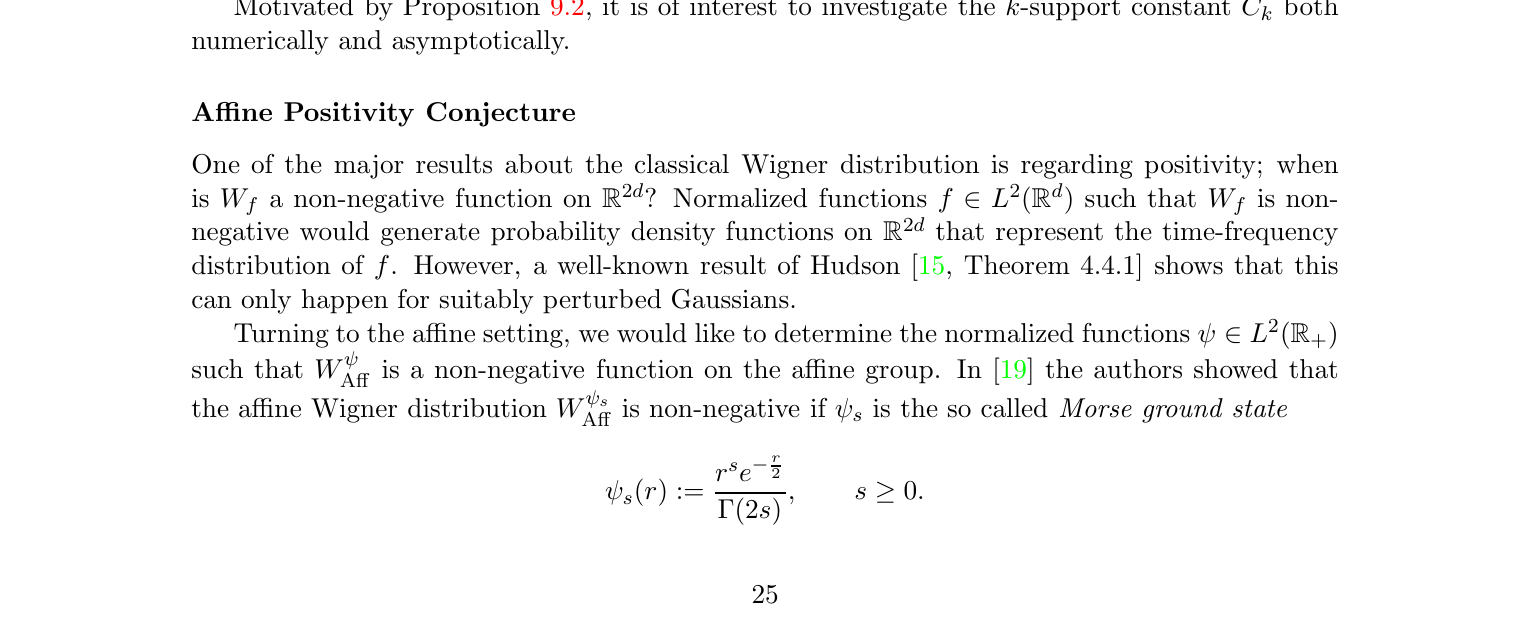
\includegraphics[width=\textwidth]{figures/open_problem_context_crop.png}

\medskip

\includegraphics[width=\textwidth]{figures/open_problem_crop.png}
\end{center}

\noindent The exact concluding statement is:
\begin{quote}
The only functions \(\psi\in L^2(\R_+)\) such that
\(\WAff^\psi\) is non-negative on the affine group are the generalized
Klauder wavelets in (9.2).
\end{quote}
Here the source uses
\(L^2(\R_+)=L^2(\R_+,dr/r)\), and its generalized Klauder wavelets are
\begin{equation}\label{eq:klauder}
  \psi(r)=C r^{-i(x+i\alpha)}e^{i(y+i b)r},
  \qquad C\in\mathbb C,\quad (x,\alpha),(y,b)\in\Aff,
\end{equation}
so \(\alpha,b>0\).

\section*{Definition and Claimed Counterexamples}

Put
\begin{equation}\label{eq:lambda}
 \lambda(u)=\frac{u e^u}{e^u-1},\qquad
 \lambda(-u)=\frac{u}{e^u-1},
\end{equation}
with the continuous value \(1\) at \(u=0\). The affine Wigner distribution
used by the source is
\begin{equation}\label{eq:awigner}
 \WAff^\psi(x,a)=\int_{\R}
 \psi\bigl(a\lambda(u)\bigr)
 \overline{\psi\bigl(a\lambda(-u)\bigr)}e^{-2\pi i x u}\,du,
 \qquad x\in\R,\quad a>0.
\end{equation}

For \(p,\beta>0\), define
\begin{equation}\label{eq:example}
 \psi_{p,\beta}(r)=N_{p,\beta}r^p e^{-\beta\sqrt r},
 \qquad
 N_{p,\beta}=\left(\frac{(2\beta)^{4p}}
 {2\Gamma(4p)}\right)^{1/2}.
\end{equation}
The chosen constant makes \(\|\psi_{p,\beta}\|_{L^2(dr/r)}=1\).

\begin{theorem}\label{thm:main}
For every \(p,\beta>0\), the function \(\psi_{p,\beta}\) in
\eqref{eq:example} belongs to \(L^2(\R_+,dr/r)\), and
\[
  \WAff^{\psi_{p,\beta}}(x,a)\geq 0
  \qquad (x\in\R,\ a>0).
\]
It is not a generalized Klauder wavelet of the form \eqref{eq:klauder}.
Consequently, the affine positivity conjecture as stated in
arXiv:1912.03112 is false.
\end{theorem}

\section*{Proof Intuition}

For each scale \(a\), formula \eqref{eq:awigner} is an ordinary Fourier
transform in \(u\). Thus it is enough to prove that its slice kernel is both
integrable and positive definite. The geometric symmetrization built into
the affine variables is especially well matched to the square root:
\[
 \sqrt{\lambda(u)}+\sqrt{\lambda(-u)}
   =\sqrt{u\coth(u/4)}.
\]
After removing the value at \(u=0\), the kernel splits into two factors. The
power factor is positive definite by Euler's product for \(\sinh\). The
square-root exponential is positive definite because
\(u\coth(u/4)-4\) is conditionally negative definite and the classical
square-root subordination formula expresses the desired factor as a positive
mixture of Schoenberg kernels. This gives positivity for an entire
two-parameter family rather than for a single numerical example.

\section*{Proof}

We use two standard notions on the additive group \(\R\). A continuous
function \(F\) is \emph{positive definite} if every matrix
\([F(u_j-u_k)]_{j,k}\) is positive semidefinite. A real even function \(q\)
with \(q(0)=0\) is \emph{conditionally negative definite} if
\[
 \sum_{j,k}c_j\overline{c_k}q(u_j-u_k)\leq0
 \quad\text{whenever }\sum_j c_j=0.
\]
We use Schoenberg's theorem: such a \(q\) is conditionally negative definite
if and only if \(e^{-tq}\) is positive definite for every \(t>0\); see
\cite[Chapter 3]{BergChristensenRessel}.

\begin{proof}[Proof of Theorem \ref{thm:main}]
The norm computation is immediate after \(t=\sqrt r\):
\[
 \int_0^\infty r^{2p}e^{-2\beta\sqrt r}\,\frac{dr}{r}
 =2\int_0^\infty t^{4p-1}e^{-2\beta t}\,dt
 =\frac{2\Gamma(4p)}{(2\beta)^{4p}}.
\]
In fact, \(x\mapsto\psi_{p,\beta}(e^x)\) is Schwartz on \(\R\), so the
example also lies in the source paper's class \(\mathcal S(\R_+)\).

Fix \(a>0\) and suppress the harmless positive normalization constant. Set
\begin{equation}\label{eq:hdef}
 h(u)=\frac{u}{2\sinh(u/2)},\qquad h(0)=1.
\end{equation}
Then
\[
 \lambda(u)=h(u)e^{u/2},\qquad
 \lambda(-u)=h(u)e^{-u/2},
\]
and hence
\begin{align}
 \lambda(u)\lambda(-u)&=h(u)^2,\label{eq:product}\\
 \sqrt{\lambda(u)}+\sqrt{\lambda(-u)}
 &=2\sqrt{h(u)}\cosh(u/4)
  =\sqrt{u\coth(u/4)}.\label{eq:sqrtsum}
\end{align}
Define the nonnegative even function
\begin{equation}\label{eq:fdef}
 f(u)=\sqrt{u\coth(u/4)}-2,\qquad f(0)=0.
\end{equation}
Dividing the slice kernel in \eqref{eq:awigner} by its positive value at zero
and using \eqref{eq:product}--\eqref{eq:sqrtsum} gives
\begin{equation}\label{eq:factorization}
 \Phi_a(u):=
 \frac{\psi_{p,\beta}(a\lambda(u))
       \psi_{p,\beta}(a\lambda(-u))}
      {|\psi_{p,\beta}(a)|^2}
 =h(u)^{2p}\exp\bigl(-\beta\sqrt a\,f(u)\bigr).
\end{equation}

We first prove that \(h^{2p}\) is positive definite. Euler's product gives
\begin{equation}\label{eq:euler}
 \frac{\sinh(u/2)}{u/2}
 =\prod_{n=1}^\infty
 \left(1+\frac{u^2}{4\pi^2n^2}\right).
\end{equation}
For every \(c,q>0\),
\begin{equation}\label{eq:gamma-mixture}
 \left(1+\frac{u^2}{c^2}\right)^{-q}
 =\frac1{\Gamma(q)}\int_0^\infty
 t^{q-1}e^{-t}e^{-tu^2/c^2}\,dt.
\end{equation}
The functions \(e^{-s u^2}\) are positive definite, so
\eqref{eq:gamma-mixture} is positive definite. Finite products of
positive-definite functions are positive definite, and the pointwise limit in
\eqref{eq:euler} is continuous at zero. Therefore
\begin{equation}\label{eq:first-pd}
 h(u)^{2p}=\prod_{n=1}^\infty
 \left(1+\frac{u^2}{4\pi^2n^2}\right)^{-2p}
\end{equation}
is positive definite.

We next prove that the exponential factor in \eqref{eq:factorization} is
positive definite. The partial-fraction expansion of \(\coth\) is
\begin{equation}\label{eq:coth-pf}
 v\coth(v/2)-2
 =4v^2\sum_{n=1}^\infty\frac1{v^2+4\pi^2n^2}.
\end{equation}
For \(c>0\), the function
\(c^2/(v^2+c^2)\) is positive definite (it is, up to a positive Fourier
normalization, the transform of \(e^{-c|x|}\)). Since its value at zero is
one,
\[
 \frac{v^2}{v^2+c^2}=1-\frac{c^2}{v^2+c^2}
\]
is conditionally negative definite. The locally uniform positive sum in
\eqref{eq:coth-pf} is therefore conditionally negative definite. Rescaling
and multiplying by a positive constant show that
\begin{equation}\label{eq:qdef}
 q(u):=2\bigl((u/2)\coth(u/4)-2\bigr)
      =u\coth(u/4)-4
\end{equation}
is conditionally negative definite and nonnegative.

Now \(f(u)=\sqrt{4+q(u)}-2\). For \(c>0\), the square-root subordination
identity
\begin{equation}\label{eq:subordination}
 e^{-c\sqrt z}
 =\frac{c}{2\sqrt\pi}\int_0^\infty
 t^{-3/2}\exp\left(-\frac{c^2}{4t}\right)e^{-zt}\,dt
 \qquad(z>0)
\end{equation}
and \eqref{eq:qdef} yield
\begin{equation}\label{eq:second-pd}
 e^{-c f(u)}=
 \frac{c e^{2c}}{2\sqrt\pi}\int_0^\infty
 t^{-3/2}\exp\left(-\frac{c^2}{4t}-4t\right)e^{-tq(u)}\,dt.
\end{equation}
By Schoenberg's theorem each \(e^{-tq(u)}\) is positive definite. The scalar
weight in \eqref{eq:second-pd} is positive and has total mass one (evaluate
at \(u=0\)). Thus \(e^{-cf}\) is positive definite for every \(c>0\).
Taking \(c=\beta\sqrt a\), both factors in \eqref{eq:factorization} are
positive definite, so \(\Phi_a\) is positive definite.

Moreover, \(0<e^{-\beta\sqrt a f(u)}\leq1\), while
\[
 h(u)^{2p}=O\bigl(|u|^{2p}e^{-p|u|}\bigr)
 \qquad(|u|\to\infty).
\]
Hence \(\Phi_a\in L^1(\R)\). The unnormalized slice kernel in
\eqref{eq:awigner} is the positive multiple
\(|\psi_{p,\beta}(a)|^2\Phi_a\), so it too is integrable and positive
definite. Bochner's theorem followed by Fourier uniqueness says that the
Fourier transform of a continuous integrable positive-definite function is a
continuous nonnegative function. Formula \eqref{eq:awigner} is precisely
that Fourier transform. Therefore
\[
 \WAff^{\psi_{p,\beta}}(x,a)\geq0
\]
for every \(x\in\R\) and \(a>0\).

Finally, the modulus of a nonzero generalized Klauder wavelet
\eqref{eq:klauder} is
\[
 |C|r^\alpha e^{-br},\qquad \alpha,b>0,
\]
whereas the modulus of \eqref{eq:example} is
\(N_{p,\beta}r^p e^{-\beta\sqrt r}\). Equality for all \(r>0\) would, after
logarithmic differentiation and multiplication by \(r\), force
\[
 p-\frac{\beta}{2}\sqrt r=\alpha-br
 \qquad(r>0),
\]
which is impossible because \(\sqrt r\) and \(r\) have different growth.
Thus the examples are not generalized Klauder wavelets.
\end{proof}

\section*{Verification Notes}

The accompanying script \texttt{code/check\_counterexample.py} independently
checks the algebraic identities, conditional-negative-definiteness matrices,
positive-definiteness Gram matrices, and FFT approximations to all affine
Wigner slices for 60 triples
\[
 p\in\{0.1,0.3,1,2.5\},\quad
 \beta\in\{0.2,1,3\},\quad
 a\in\{0.05,0.3,1,5,20\}.
\]
Run it from the repository root with
\begin{verbatim}
conda run --no-capture-output -n sandbox python \
  runs/fa_banach_001/solutions/counterexamples/\
  1912.03112_affine_wigner_sqrt_exponential_positive/\
  code/check_counterexample.py
\end{verbatim}
The finite tests are diagnostics only. Positivity for all parameters and all
phase-space points follows from the positive-definiteness proof above.

\section*{Novelty and Limitations}

A bounded check on August 9, 2026 searched the run's registry, solution,
attempt, and proof-gap indexes and used arXiv-focused web queries for the
paper/arXiv id, the exact phrase \emph{Affine Positivity Conjecture},
combinations of \emph{affine Wigner}, \emph{nonnegative},
\emph{generalized Klauder}, and \emph{counterexample}, and the
square-root-exponential family. It found the source paper and older background
on positive Morse/Klauder states, but no later explicit resolution and no
prior appearance of this counterexample family. The search was bounded and
cannot establish priority. The claimed mathematical statement is exactly a
disproof of the source conjecture; it does not attempt a replacement
classification of all nonnegative affine Wigner states.

\section*{Human Review Recommendation}

Send to expert review as a full counterexample. The most useful adversarial
checks are: (i) the constants in \eqref{eq:coth-pf} and \eqref{eq:qdef};
(ii) the square-root subordination formula \eqref{eq:subordination}; and
(iii) the use of Bochner plus \(L^1\)-integrability to upgrade the representing
positive measure to the pointwise nonnegative Fourier transform.

\begin{thebibliography}{9}

\bibitem{BergeBergeLuef}
E. Berge, S. M. Berge, and F. Luef,
\emph{The Affine Wigner Distribution},
arXiv:1912.03112, 2019.

\bibitem{BergChristensenRessel}
C. Berg, J. P. R. Christensen, and P. Ressel,
\emph{Harmonic Analysis on Semigroups: Theory of Positive Definite and Related
Functions}, Graduate Texts in Mathematics 100, Springer, 1984.

\end{thebibliography}

\end{document}
